\documentclass[11pt]{exam}
\usepackage{tikz}
\usetikzlibrary {plotmarks}
\usepackage{multicol}
\usepackage{subfigure,amsmath,amssymb}
\usepackage{systeme}

\newcommand{\class}{MATH 96}
\newcommand{\term}{Spring 2025}
\newcommand{\examnum}{Exam 3 v.1.} 
\newcommand{\examdate}{4/23/2025}
\newcommand{\timelimit}{60 Minutes}

\parindent 0ex

\begin{document} 

\pagestyle{head}
\firstpageheader{}{}{}
\runningheader{\class}{\examnum\ - Page \thepage\ of \numpages}{\examdate}
\runningheadrule

\begin{flushright}
\begin{tabular}{p{2.1in} r l}
\textbf{\class} & \textbf{First and Last Name:}     & \makebox[2.2in]{\hrulefill}\\
\textbf{\term}  &                    &\\
\textbf{\examnum} &  & \\
 & \textbf{Section:} & \makebox[2.2in]{\hrulefill}\\

\end{tabular}\\
\end{flushright}
\rule[1ex]{\textwidth}{.1pt}

This exam contains \numpages\ pages (including this cover page) and
\numquestions\ problems.  Check to see if any pages are missing.  Enter
your name and your section above.
\vspace{0.2in}

You may \emph{not} use textbooks, course notes, cell phones, or calculators during this exam.
\vspace{0.2in}

You are required to show your work on each problem on this exam, and the following rules apply:
\vspace{0.2in}

\begin{minipage}[t]{3.7in}
\vspace{0pt}
\begin{itemize}

\item \textbf{Organize your work in a reasonable, neat, and coherent way.} Work that is jumbled, disorganized, or lacks clear reasoning will receive little credit.  

\item \textbf{Partial credit may be given.} Any answer must be supported by calculations, explanation, and/or algebraic work to receive full credit.  Unsupported answers will not receive full credit, but well-argued, incorrect solutions may earn partial credit.

\item \textbf{If you require more space, use the back of a page.} Clearly indicate when you do this below the problem.
\end{itemize}

Do not write in the table to the right.
\end{minipage}
\hfill
\begin{minipage}[t]{2.3in}
\vspace{0pt}
\gradetablestretch{2}
\vqword{Problem}
\addpoints
\gradetable[v][pages]
\end{minipage}
%=======================================================================================================================
%=======================================================================================================================
\newpage
\begin{questions}

%=======================================================================================================================
\question[20] Find solutions to the given quadratic equations by any appropriate method.
\noaddpoints
\vspace{2pt}
\begin{parts}
\part[10] $x^2 = -4x + 5$
\vspace{2in}
\part[10] \(3x^{2}-7x +2 =0\)
\vspace{2in}
\end{parts}
\addpoints

\question[10] Simplify the following expressions. ($x$, $y$, and $z$ are non-negative.)
\noaddpoints
\vspace{2pt}
\begin{parts}

\part[5] $\displaystyle \sqrt{ \frac{36x^4y^2}{9x^2y^8} }$
\vspace{1.5in}

\part[5] $\sqrt[3]{27 x^{12} y^6 z^9}$
\vspace{2in}
\addpoints
\end{parts}

\question[10] Find a polynomial expression that represents the area of the figure below. \emph{Fully expand your polynomial answer.}
\begin{figure}[h!]
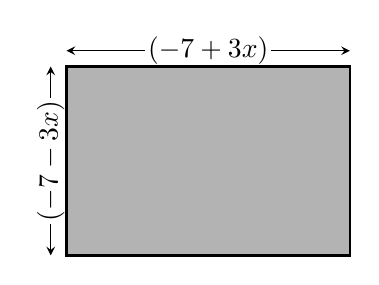
\begin{tikzpicture}[scale=0.4]
\fill[gray,fill opacity=0.6] (-4.5,3)--(4.5,3)--(4.5,-3)--(-4.5,-3)--cycle;
\draw[-,thick] (-4.5,3)--(4.5,3)--(4.5,-3)--(-4.5,-3)--cycle;
\node[rotate=90] at (-5,0) {$(-7-3x)$};
\draw[-stealth] (-5,2)--(-5,3);
\draw[-stealth] (-5,-2)--(-5,-3);
\node at (0,3.5) {$(-7+3x)$};
\draw[-stealth] (2,3.5)--(4.5,3.5);
\draw[-stealth] (-2,3.5)--(-4.5,3.5);
\end{tikzpicture}
\end{figure}
\addpoints

\question[20] Expand the following expressions.
\noaddpoints
\vspace{2pt}
\begin{parts}
\part[10] $(3x - 2)(x + 4)(2 - x)$
\vspace{2in}

\part[10] $(m - 2)(m^2 + 2m + 4)$
\vspace{2in}
\end{parts}
\addpoints

\question[10] Convert the following expressions to radical form and simplify if possible. 
\noaddpoints
\vspace{2pt}

\begin{parts}
\begin{multicols}{2}
\part[5] $81^{\frac{3}{4}}$
\part[5] $(-27)^{\frac{2}{3}}$  
\end{multicols}
\end{parts}
\vspace{2.5in}
\addpoints

\question[20] Perform the indicated operations. \emph{Simplify the expression as much as possible.}
\noaddpoints
\vspace{2pt}
\begin{parts}
\part[10] $\displaystyle 5\sqrt{2} - 2\sqrt{50}$
\vspace{2in}

\part[10] $\left( \sqrt{16x^4y^2} \right) \cdot \left( 2xy\sqrt{9x^2y^6} \right)$
\vspace{2in}
\end{parts}
\addpoints

\question[10] Divide the expression $(x^3 + 2x^2 - 5x + 6) \div (x - 1)$ and find the quotient and the remainder.
\addpoints
\vspace{3.2in}

Quotient: \hfill Remainder: \hspace{2in}

\end{questions}
\end{document}


